\section{User Interface}
\label{user-interface}

We decided to use a Material Design library \cite{Elm-lang-material-design} for
most of the user interface. Material Design is a design system developed by
Google \cite{Material-design}, which we used to create menus, buttons, layouts,
and more for the parts of the editor that we just wanted functioning. Some
sample configurations are in figure \ref{fig:final_ui}, which we will dicuss
more in this section.

We wanted more control over the appearance of the editor expression builder and
visualizing ASTs. In this section we discuss different approaches and ideas to
visualize ASTs and use the editor and editor interface. The discussion does not
aim to provide an interaction-design aspect, but general reflection upon the
projects outcome and potential pitfalls from a usability and functionality
minded aspect.

\subsection{Visualizing ASTs and editor expressions}

We implemented the two visualizations described in section \ref{design}, i.e. a
textual representation and a tree representation. The implementation of the
textual representation was simply to convert our AST data structure to HTML,
which is quite straightforward \elmhtml. To make it less monotone and
unmanageable, we added syntax highlighting with some custom CSS we wrote
specifically for this. The last image in figure \ref{fig:final_ui} shows this.

The implementation of the tree representation was a bit more involved. We
considered a few different web technologies for this representation. We could
use HTML and CSS to create a tree view, but we decided against this in favor of
web technologies that are more geared towards graphics. We have two options for
rendering graphics in the browser, which are SVG \cite{svg} and WebGL
\cite{webgl}. We ended up choosing SVG as it is easier to work with in Elm, but
also because WebGL seems a bit overkill for this purpose. The first two images
in figure \ref{fig:final_ui} show some trees. As seen in the images, the cursor
is not shown as a node in the AST, but rather highlights the node at which the
cursor rests. Compared to our first design approach - the one seen in figure
\ref{fig:ast_visual_tree} - this new approach makes cursor movement much
smoother to concieve since the tree structure is not changed whenever the cursor
is moved.

The visualization of the editor expression builder was similar to the textual
representation of ASTs. We implemented a function that given an \texttt{Edt}
returns HTML, which we discussed the details of in section \ref{modeling}.
Finally, we styled the editor expression builder with CSS. An example of an
editor expression being built is in the upper left corner of the images in
figure \ref{fig:final_ui}.

\subsection{User interface features}

Since the editor is quite different to most editors, there are some constrains
that make features that most would expect difficult or impossible to implement.
A usability constraint we have with both visualizations, is that we will not be
able to simply click on a node and move the cursor there. This is because
navigation is only defined for one child or parent at a time, and we cannot move
to any arbitrary node. As such, we have to move through the AST one child or
parent at a time.

We did however add other features to the tree view to make the editor more
usable. To get a better workflow when using the tree view, we have implemented
zoom functionality, making it possible to zoom in on the area being worked on,
or zooming out to get a better overview of the full AST. Likewise we
have made it possible to look at different parts of the AST, moving the AST by
clicking and dragging the mouse around in the AST view section.

\begin{figure*}
  \center
  \noindent\begin{minipage}{\textwidth}
    \center
    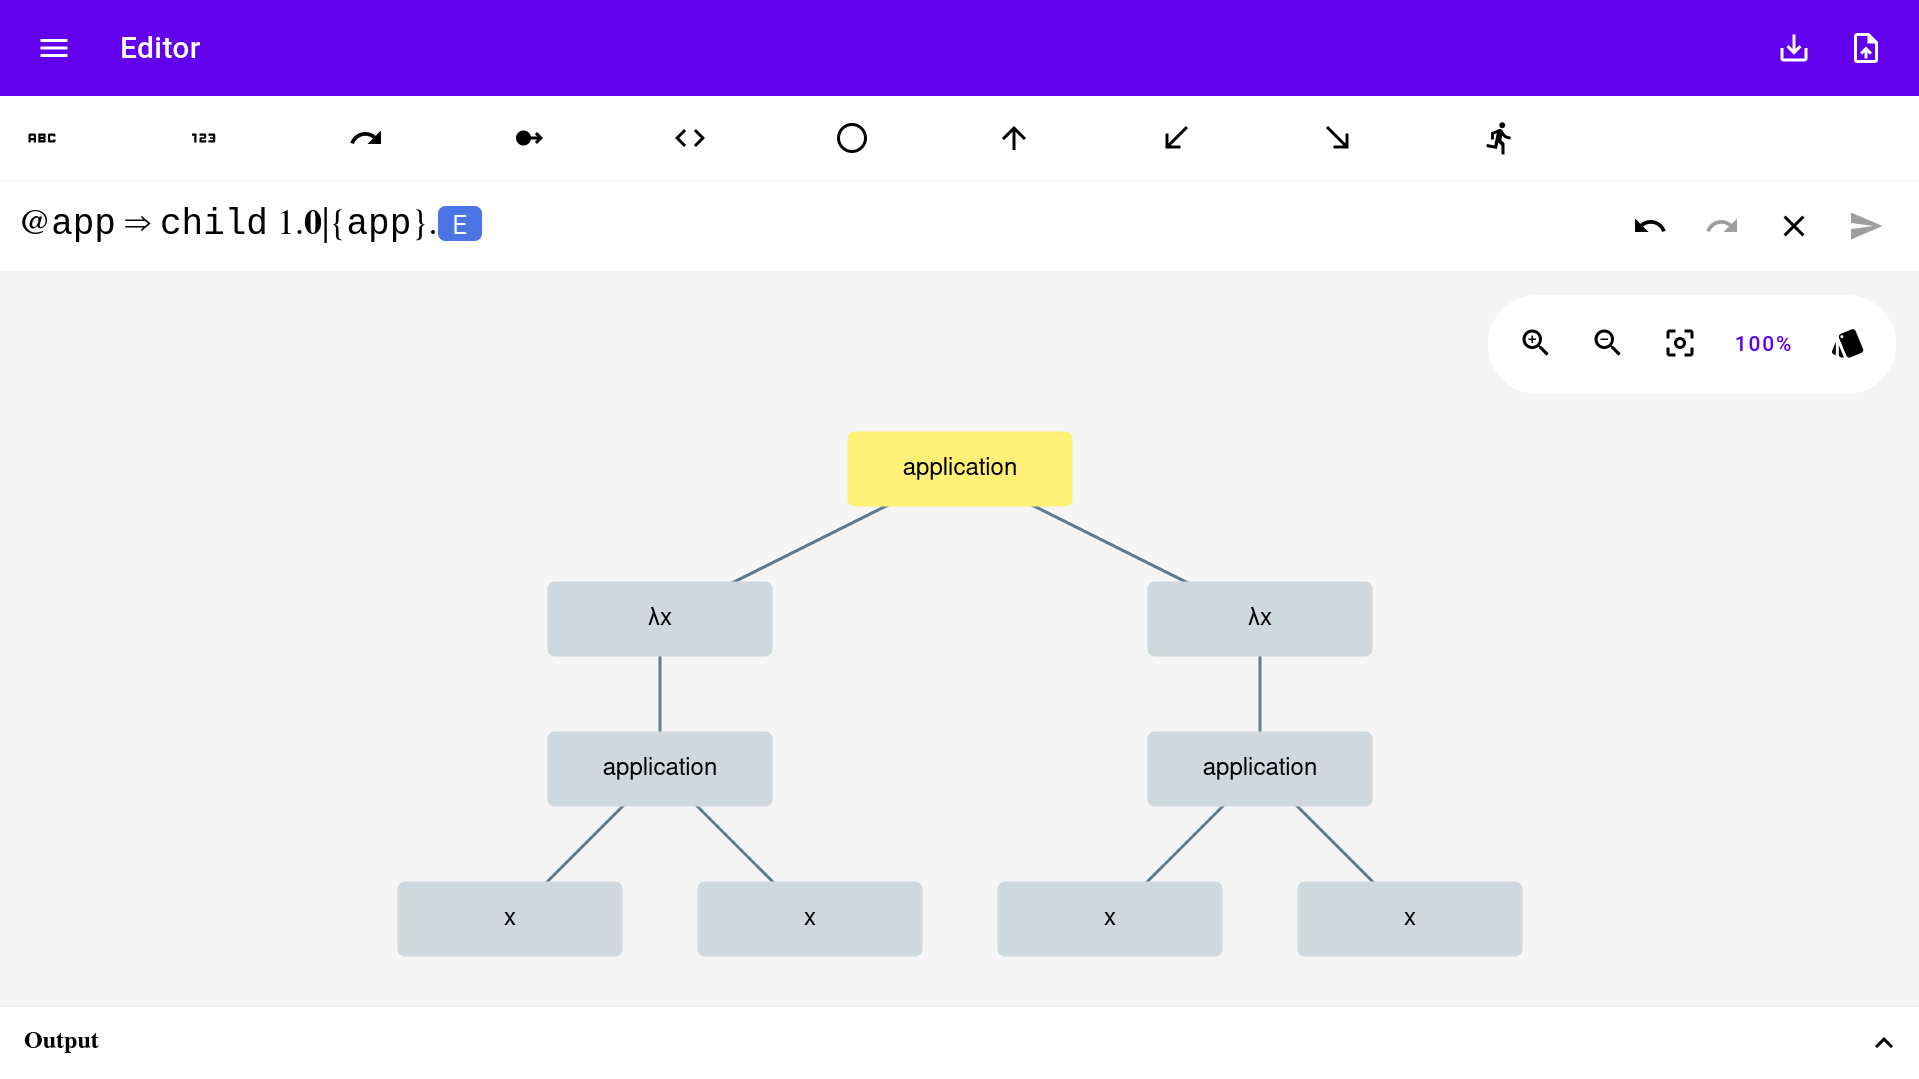
\includegraphics[width=0.7\textwidth]{assets/final_ui1.png}
  \end{minipage}\hfill
  \begin{minipage}{\textwidth}
    \center
    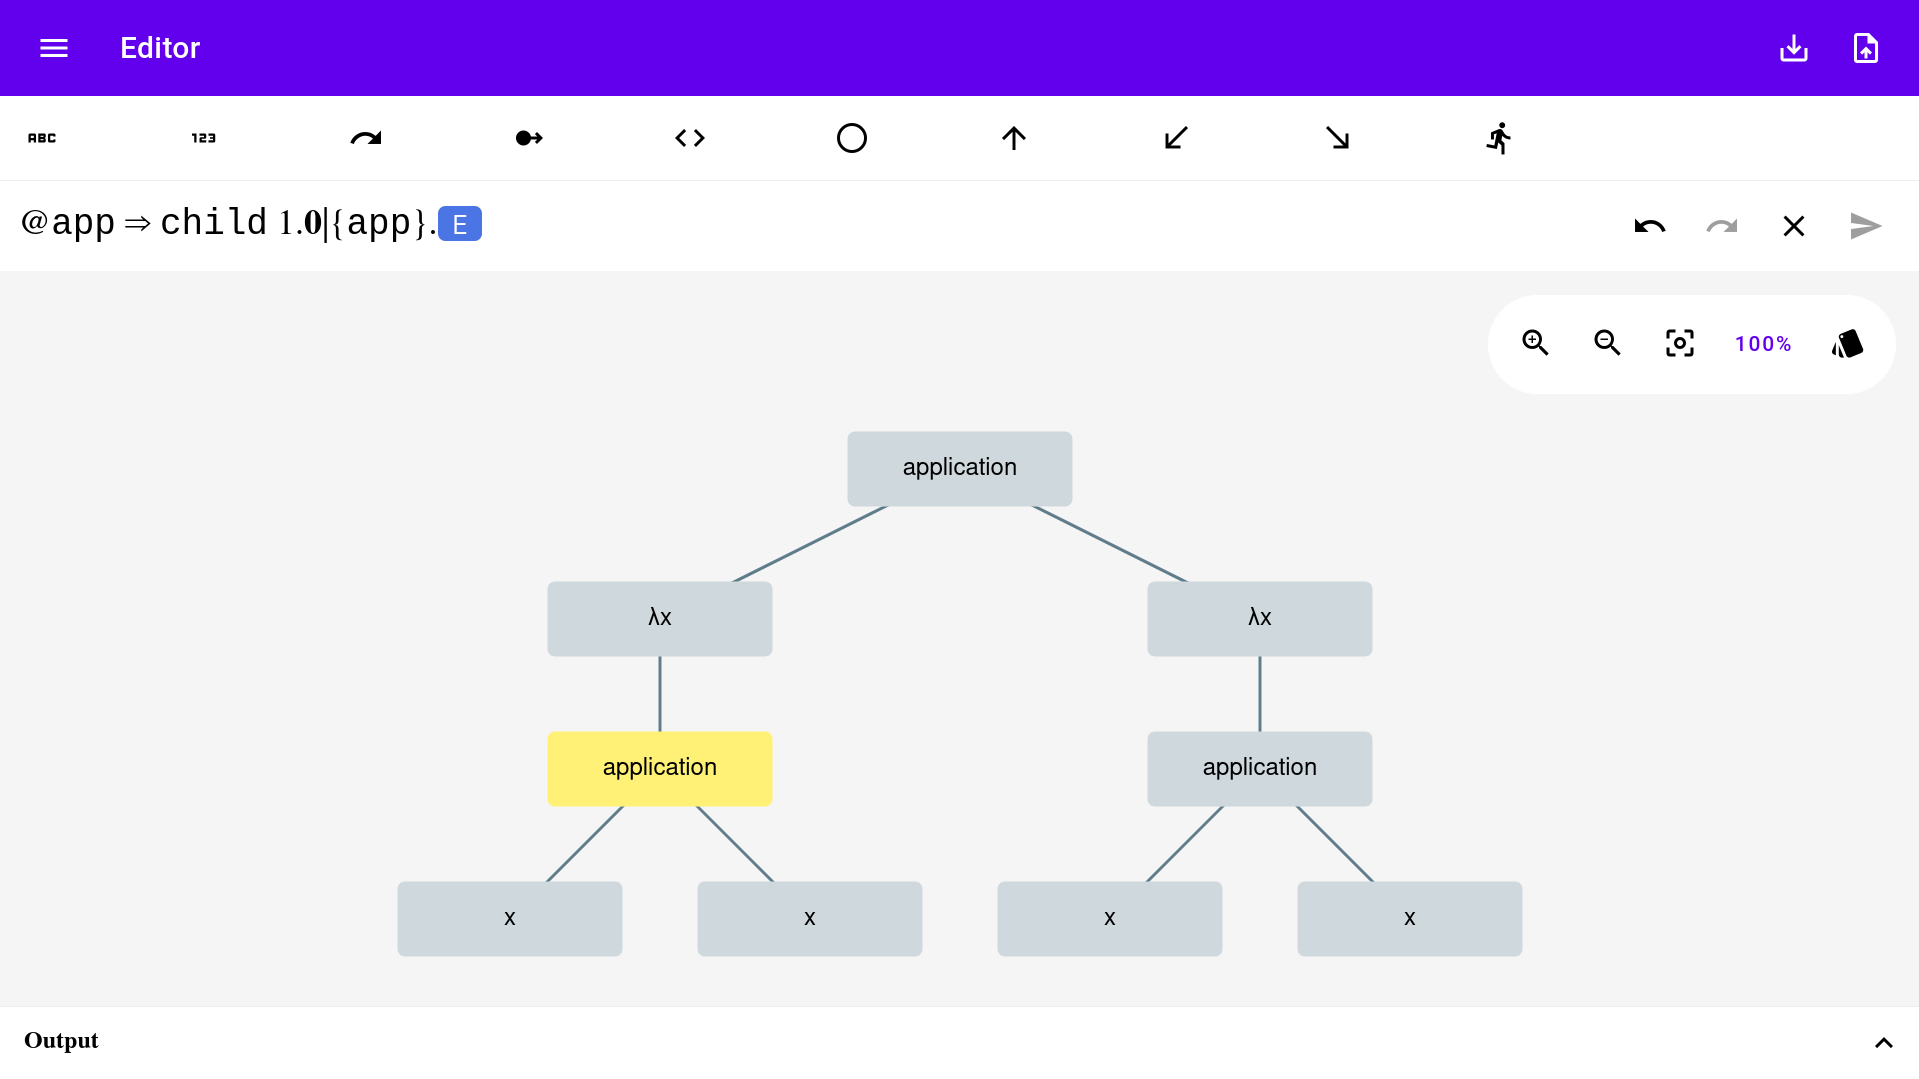
\includegraphics[width=0.7\textwidth]{assets/final_ui2.png}
  \end{minipage}\hfill
  \begin{minipage}{\textwidth}
    \center
    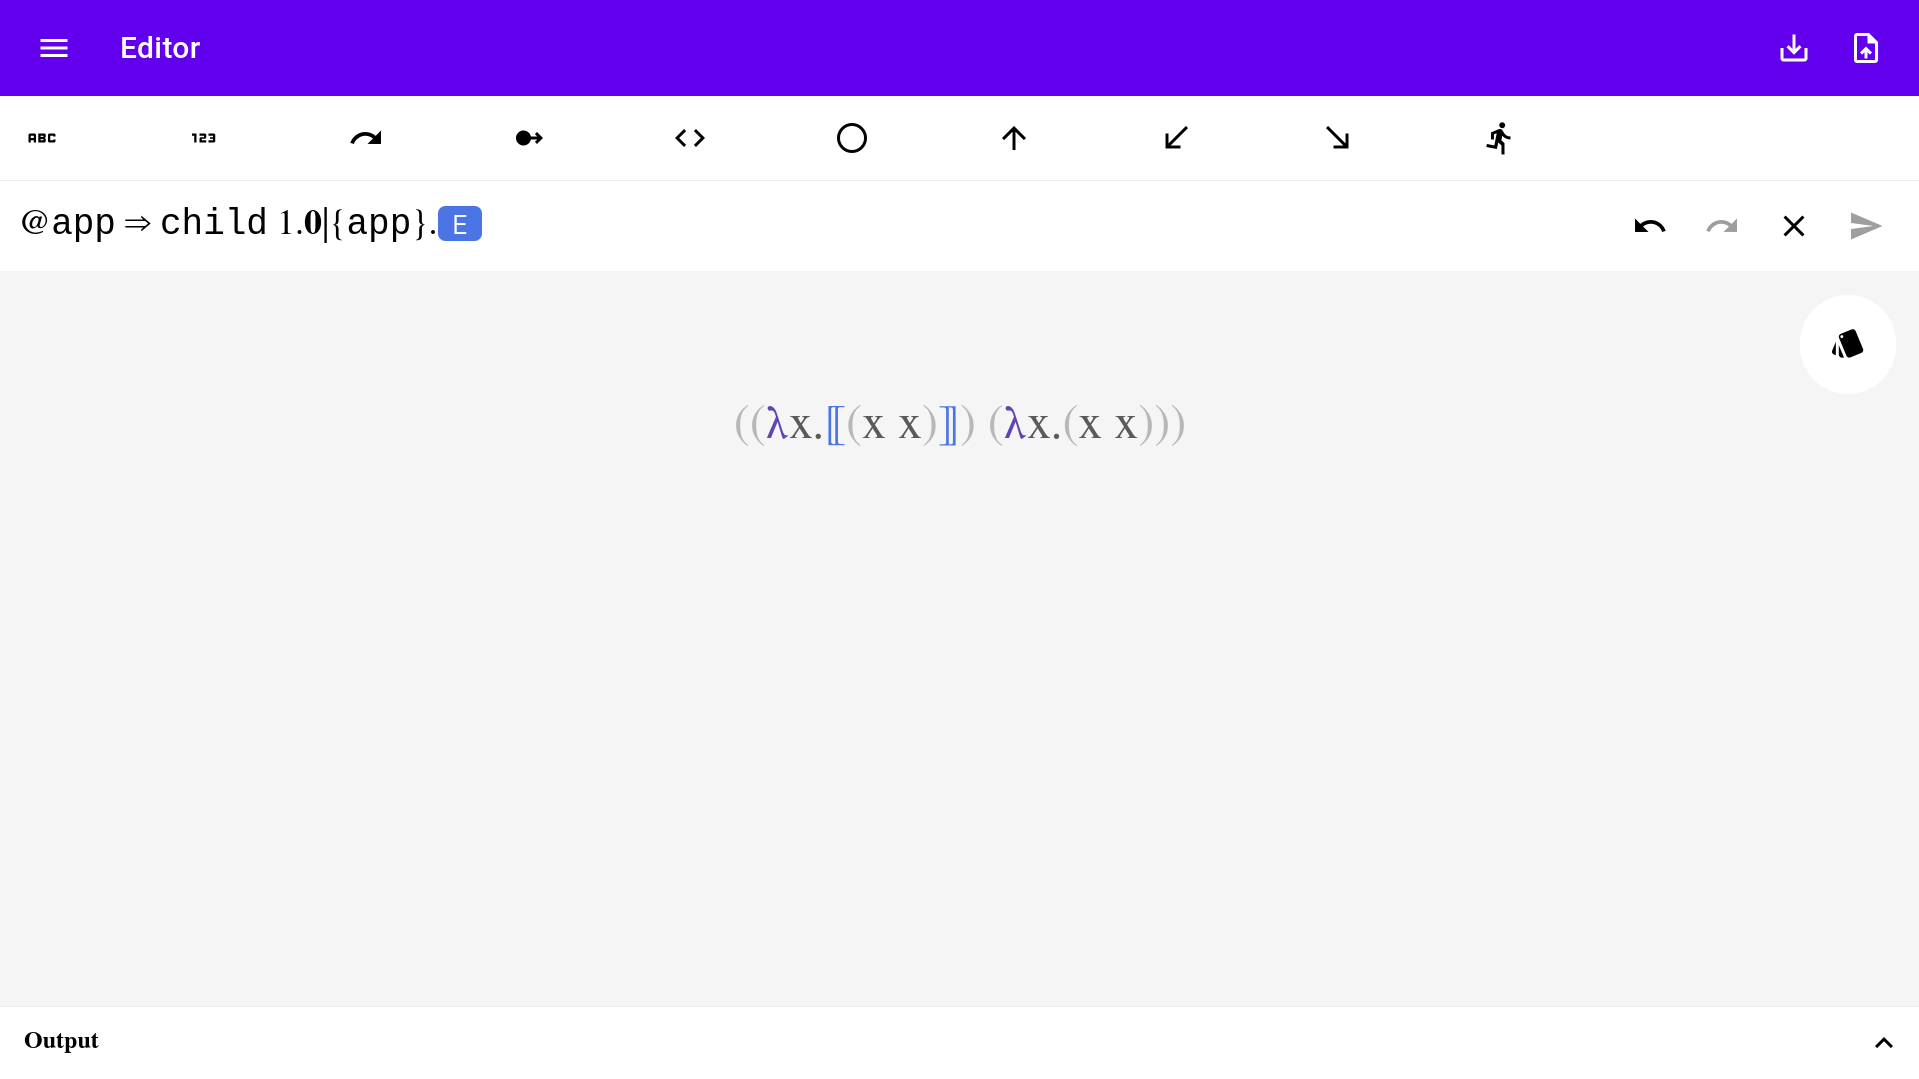
\includegraphics[width=0.7\textwidth]{assets/final_ui3.png}
  \end{minipage}\hfill
  \caption{The figures \ref{fig:ast-in-text-form} and \ref{fig:ast_visual_tree} from section \ref{design} recreated in the final UI}
  \label{fig:final_ui}
\end{figure*}
